\chapter{Programming Snippets}

\section{Hello World Snippet}
The first snippet shows how to simple transfer data synchronously to the GPU global memory and manipulate it with a kernel. It's a good place to start with and to check whether your installation of the cuda toolkit and nvidia drivers work as expected.\\

It simply moves a character to the GPU memory and manipulates it to change the "CPU" string to a "GPU" string, which will be read back and written to the console.


\section{Create Random Matrix File}
The second snippet won't do anything on the GPU. But for testing with kernels it's handy to have some files with matrices to compute. This Snippet provides the means to create, store such matrices, as well as write them to the console. For unknown reasons it's not possible to create matrices that are bigger as 1000x1000 elements.

\section{Matrix Multiplication}
The third snippet performs a first matrix multiplication kernel that computes the matrix multiplication out of the global memory of the GPU. Furthermore it compares the result to a algorithm that performs the same multiplication on the CPU. You will see, that the CPU performs faster for small matrices because there's no need to transfer the data to the GPU.\\

You will also see, that the maximal size of the matrix that can be calculated on the GPU is limited. This is due to the fact that in this snippet (for simplicity) we use only one block and this block is limited to 1024 Threads, that means we can only calculate matrices with up to 1024 elements (Depending on the GPU it might be less or even up to 2048).


\section{System Info Readout}
In order to write an optimal kernel for the given hardware it is essential to know some specifications of the GPU. This snippet provides the means to read out the important ones and store those inside a file.\\

Particularly we're interested in the following specs that are described below.\\

\subsection{Clock Rate}
This is the computing unit clock rate and defines the speed for calculations. It's in the area of MHz which doesn't seem very fast, but remember we do have tons of computing unit in parallel.

\subsection{Number of Streaming Multiprocessors}
A streaming multiprocessor is a collection of computing units called a Warp. It processes multiple given blocks. Actual GPUs can process up tu 8 blocks in "parallel". Parallel is hear in quotes because it contains a limited number of computing units which can work really in parallel, the rest of the threads will be executed in serial batches of those parallel executable threads.

\subsection{Number of Cuncurrent Kernels}
This parameter specifies how many different kernels can be executed by the GPU at the same time.

\subsection{Warp Size}
As mentioned in the Streaming Multiprocessor section a SM has one Warp that are 32 (in most actual GPUs) concurrent processing units. As the GPU doesn't have a hardware pipeline for executing commands efficiently it simply calculates another batch of data while waiting for time consuming instructions like memory loads, memory stores, branches etc. Therefor it is crucial to provide enough threads to a streaming multiprocessor in order to fully utilize the computing units. Remember a load/store instruction to the global memory needs about 100 cycles whereas a floating point instruction only needs one. When analyzing a kernel one often counts the number of global memory accesses as well as the number of floating point operations and creates the compute-to-global-memory-access ratio. 

\subsection{Total Global Memory}
This parameter describes the maximum random access memory of the GPU. This memory is the biggest one and is the only one that the host CPU can send data to. This means CPU, as well as all Cores of the GPU have read and write access permission to it so synchronization is an issue with this type of memory.

\subsection{Total Constant Memory}
The constant memory is a read only memory for the GPU. The host CPU can initialize this constant memory prior to calling a kernel with special API functions. All data stored into the constant memory will be load into the L2-Cache of each streaming multiprocessor. Therefor it's always available like a global variable inside the kernel and very fast. Even faster than shared memory but slower than the registers.

\subsection{Shared memory per Block}
The hardware of the streaming multiprocessors contains on chip memory called Shared Memory. This kind of memory is way faster than the global GDDR5 memory. But only the streaming multiprocessor has read/write access to it. This means that the kernel has to copy the data from the global memory to the shared memory. As memory requires a lot of chip-space it's also a very expensive resource. That's why it not very big.\\

\subsection{Memory Pitch}
The global memory of a GPU may consist of multiple memory controllers which each manages a portion of the whole memory. The pitch describse how big such a portion is.

\subsection{Max Threads per Block}
A streaming multiprocessor is in its capability also limited in the number of maximal threads to handle, not only the number of blocks. This is due to the hardware indexers. Therefor it exists a maximal number of thread a SM can handle in each dimension (X,Y,Z) and as a whole.

\subsection{Max Blocks per Grid}
Similar to the max threads per block, there exists a maximal number of blocks an SM can handle. This number is usually very big and not limiting. \\
Remember this number has nothing to do with the parallel computation capabilities of the GPU. The number of SM, the Clock and the Warp size divine that. The Max Blocks per Grid can be interpreted as a maximal queue length for blocks waiting to be computed by the SMs.

\subsection{Max Registers}
This number describes the total count of registers that are available inside a streaming multiprocessor. This resource is shared between all the Treads of a block, not all the thread inside a warp to enable fast switching between different warp sets. So pay attention that the register memory won't limit the number of threads/blocks that can reside inside a streaming multiprocessor.


\section{Matrix Calculation using Blocks}
To be able to compute bigger matrices than the maximal number of threads per block we obviously need multiple blocks. This snippet shows how to declare a grid of blocks and how to use the block index hardware signal to address the correct data portion to process.


\section{Matrix Calculation using Shared Memory}
As we have seen in the GPU Architecture part that a streaming multiprocesser contains on-chip-memory which is way faster than the global memory we want to use that to minimize global memory access. This snippet shows how to split the data into small portions called tiles. For those tiles memory will be allocated inside the kernel and the input data from the global memory will be copied into the shared memory of the tile.


\section{Matrix Calculation using Constant Memory}
The last type of memory we can access is the fast constant memory. This snippet shows an example how to access it.
\pagebreak

\section{Comparing different Methods for Image Substraction}
It's a common task to remove a background light intensity of a camera image. Therefore this snippet shows how tho subtract a vector from each row of an image efficiently.

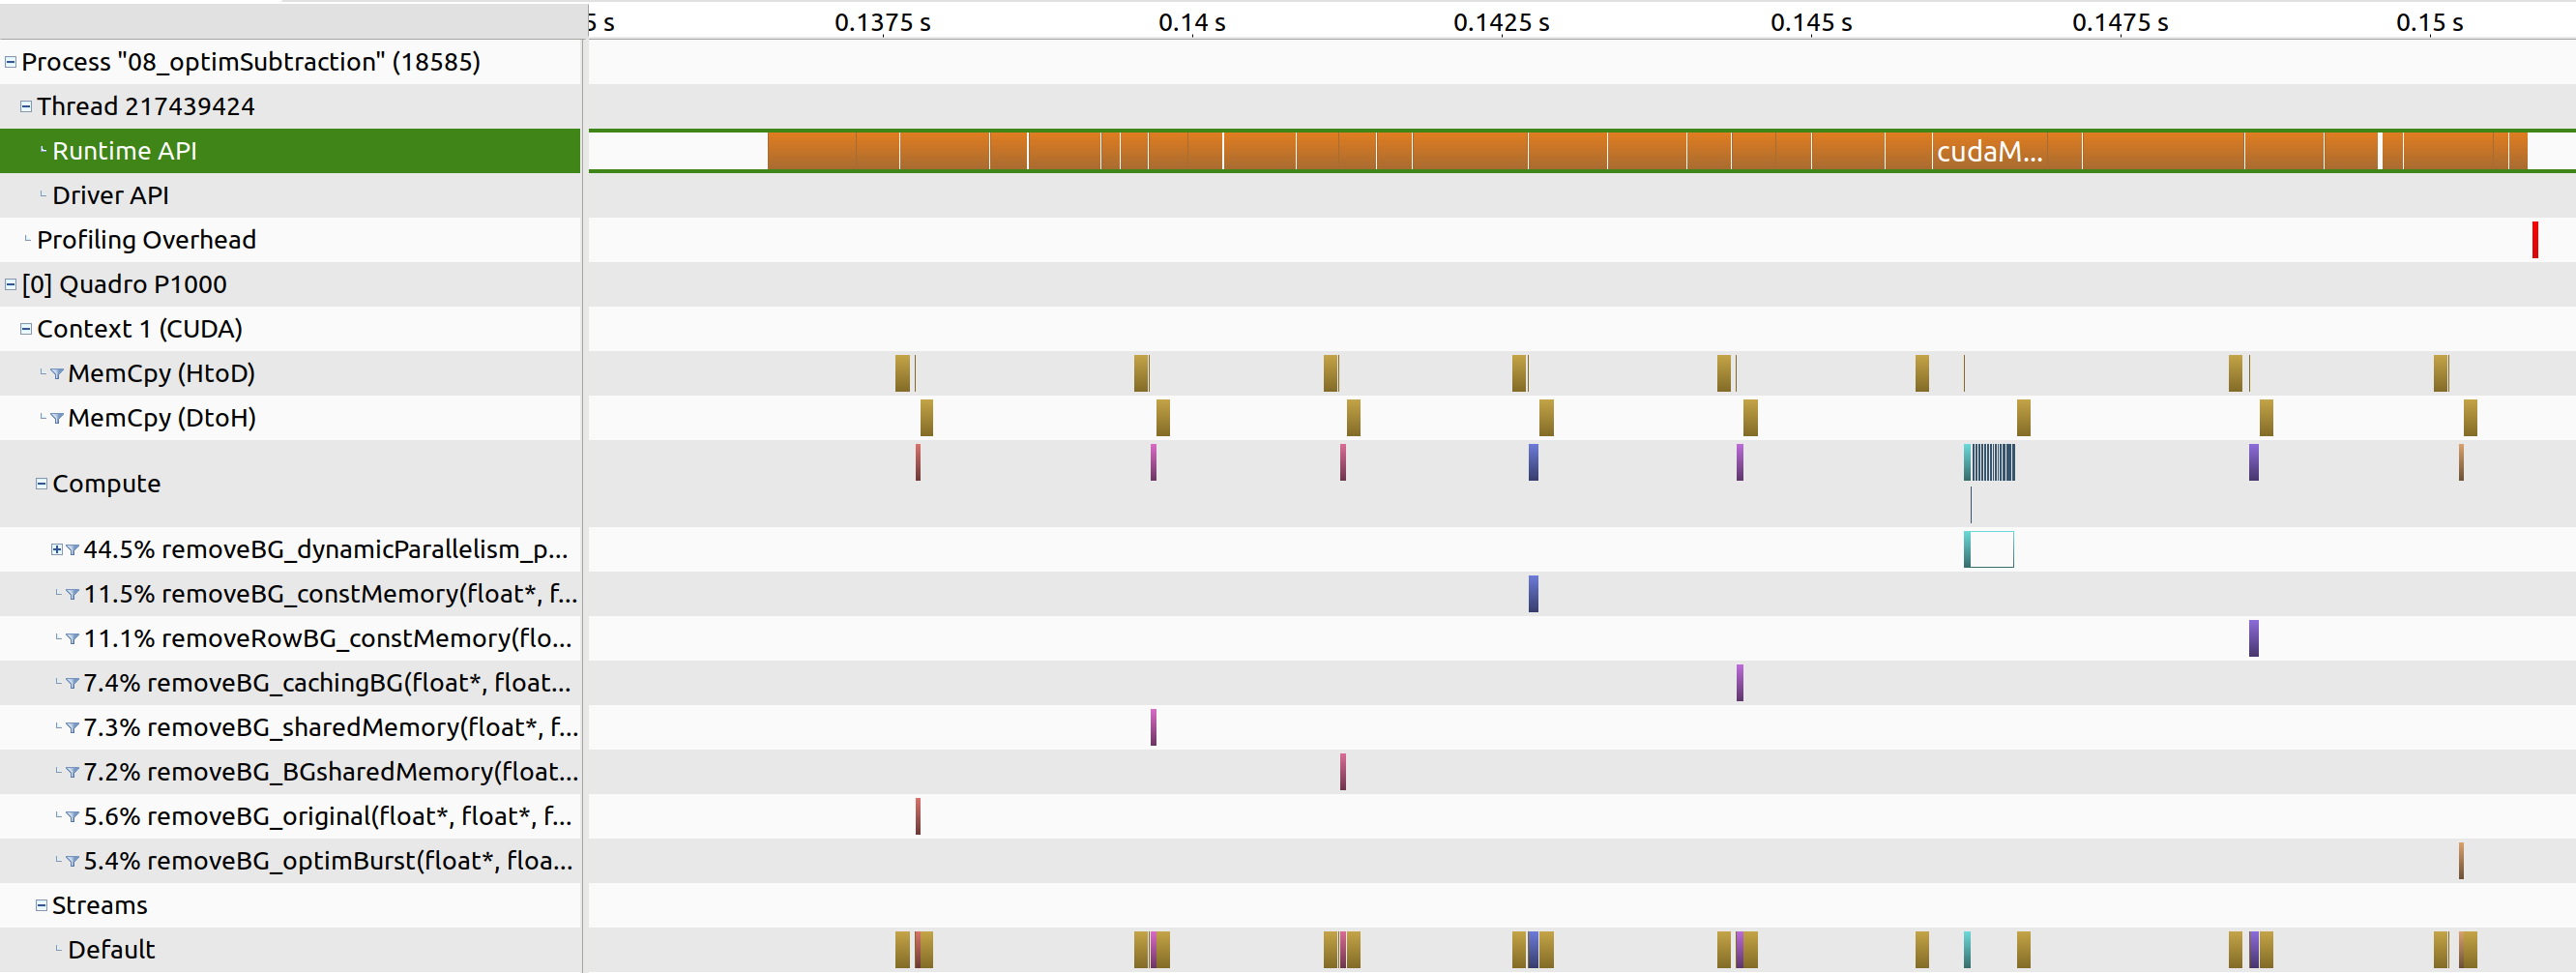
\includegraphics[width=\textwidth]{imgs/compareBGremoval.png}

As it can be seen by the analysis it's not possible to speed up this kind of kernel though shared memory. The constant memory approach doesn't help much neither because the vector isn't very big, so it will be stored inside the cache anyway.\\
So the only thing speeding up this kind of kernel are optimal burst transfers. The burst transfers are already very optimal in the original kernel, that's why the optimBurst kernel is only slightly better.


\section{Memory Types Demonstration}
This snippet shows how to prepare the host memory for best possible transfer speeds.


\section{Simple Asynchron Memory transfer Example}
Streams are the tool of CUDA to enable asynchronous (interleaved) data transfer from host memory to GPU memory. This snippet shows how to create streams and assign kernels to the streams.\\
In the examples before we used a stream to, but it was hidden. We used the default stream which is always synchronous.
\cite[CUDA Programming Guide, chapter 3.2.5.5ff]{cudaGuide}
\pagebreak

\section{Asynchron Memory transfer Class}
This snippet implements a streamer class that creates a stream and manages the data transfers and kernel executions.\\
When analyzing the code with the nvidia-profiler tool we see that data transfers and kernel execution ar the smallest part of the whole execution time. In the next snippet we're this will be corrected.\\

The output of the nvidia-profiler:\\
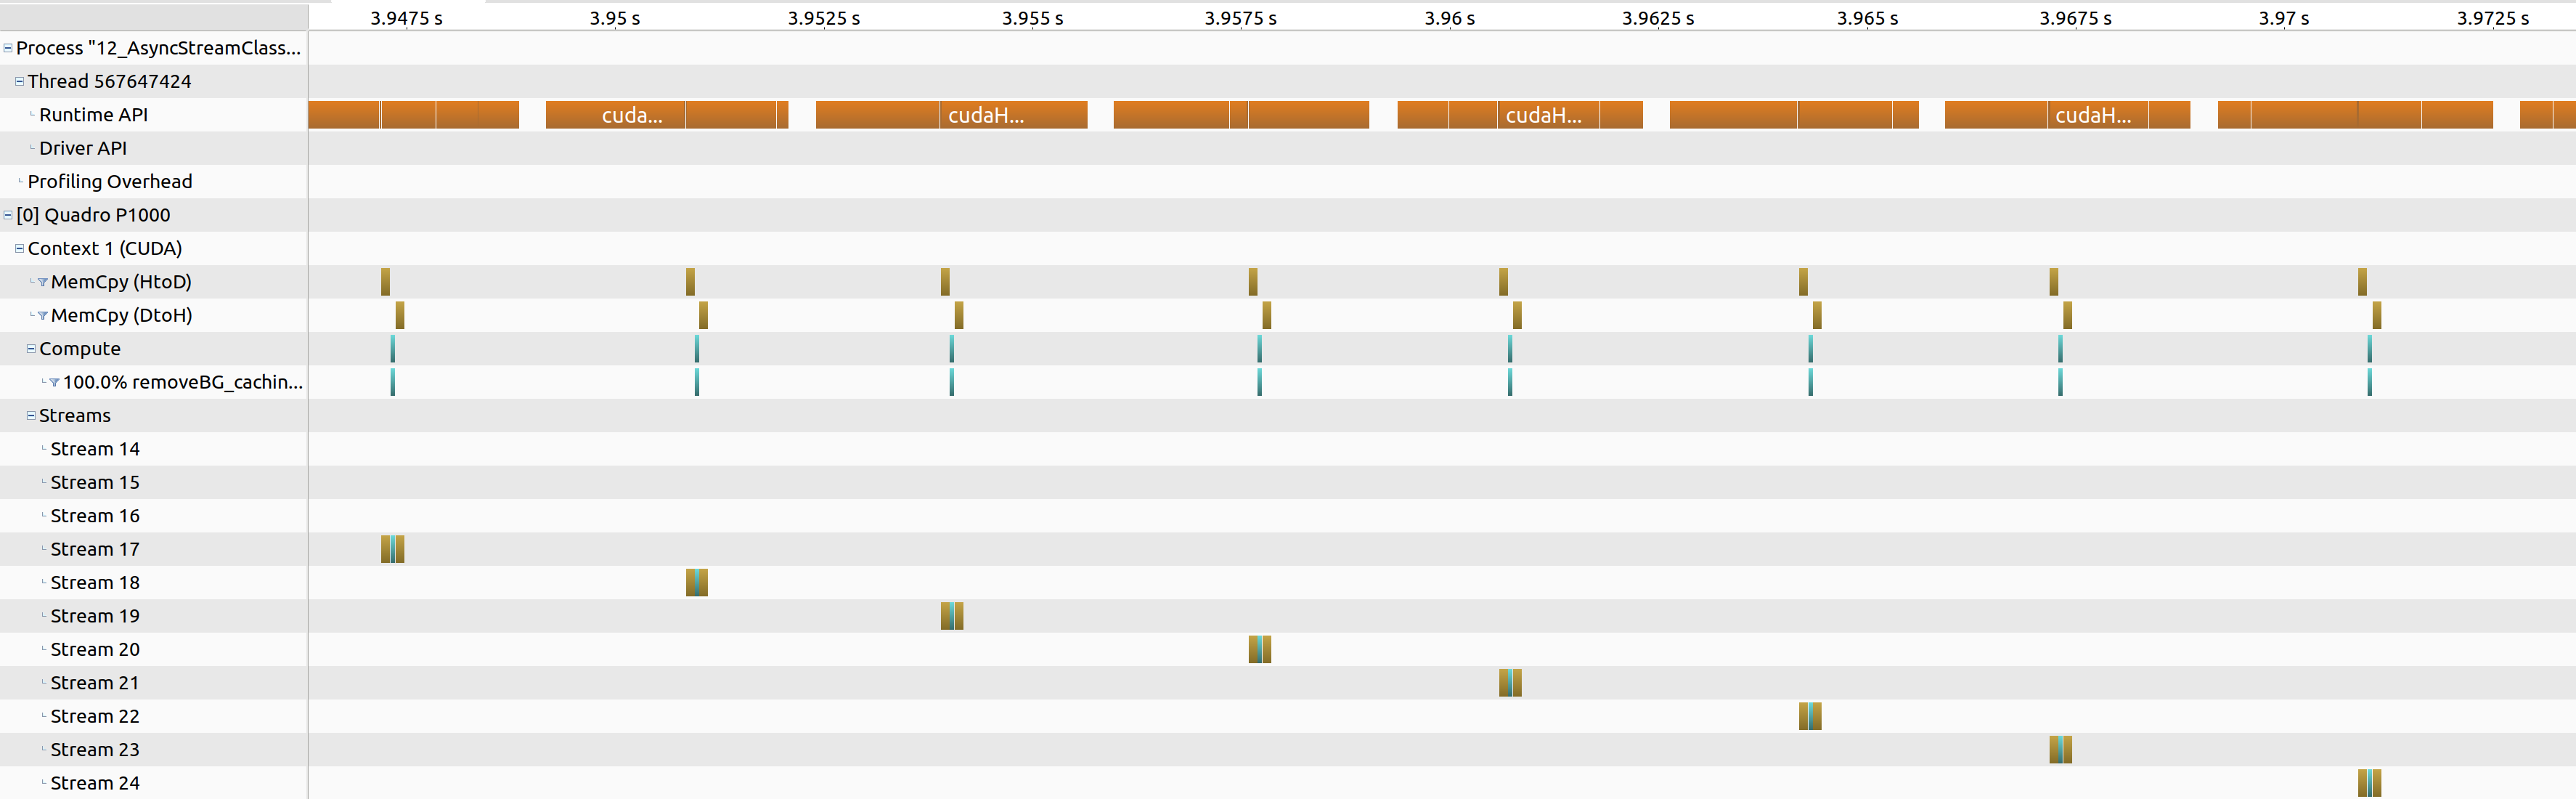
\includegraphics[width=\textwidth]{imgs/StreamsSlow.png}

We can see now, that the kernels indeed execute in different streams concurrently. But the main time is used for allocation etc, so it's not more efficient than the sequential kernel execution.

Output readings:\\
\begin{tabular}{ll}
	cudaHostRegister input image: & 403us \\
	cudaMalloc input image: & 213us\\
	cudaHostRegister output image: & 843us\\
	cudaMalloc output image: & 193us\\
	memCopy input image: & 50.5us\\
	kernel: & 193us\\
	memCopy output image: & 50.5us\\
	cudaHostUnregister input image: & 580us\\
	cudaFree input image:& 136us\\
	cudaHostUnregister output image: & 359us\\
	cudaMalloc output image: & 140us\\
\end{tabular}

We can calculate the theoretical throughput for BScans with 640 A-Scans per BScan: $C = \frac{1}{2*50.5us + 192us} * 512 \approx 1.7M$ AScans per second.\\
But we lose a lot of time with allocation and memory pinning in this implementation which limits us to 160k AScans per second.
\cite[CUDA Programming Guide, chapter 3.2.5.5ff]{cudaGuide}
\pagebreak


\section{Improved Streamer Class}
As it was shown in the Streamer class section the streamer class needs improvement. By allocating the device memory just once for the input and output image per stream and using already pinned memory on the CPU side it was possilbe to improve the class a lot!

Output readings:\\
\begin{tabular}{ll}
	memCopy input image: & 118us\\
	kernel: & 57us\\
	memCopy output image: & 154us
\end{tabular}

This results in full bandwidth usage of the PCI bus and a speed of: $C = \frac{1}{118+57+154} * 512 = 1.55$MAScans per second. 

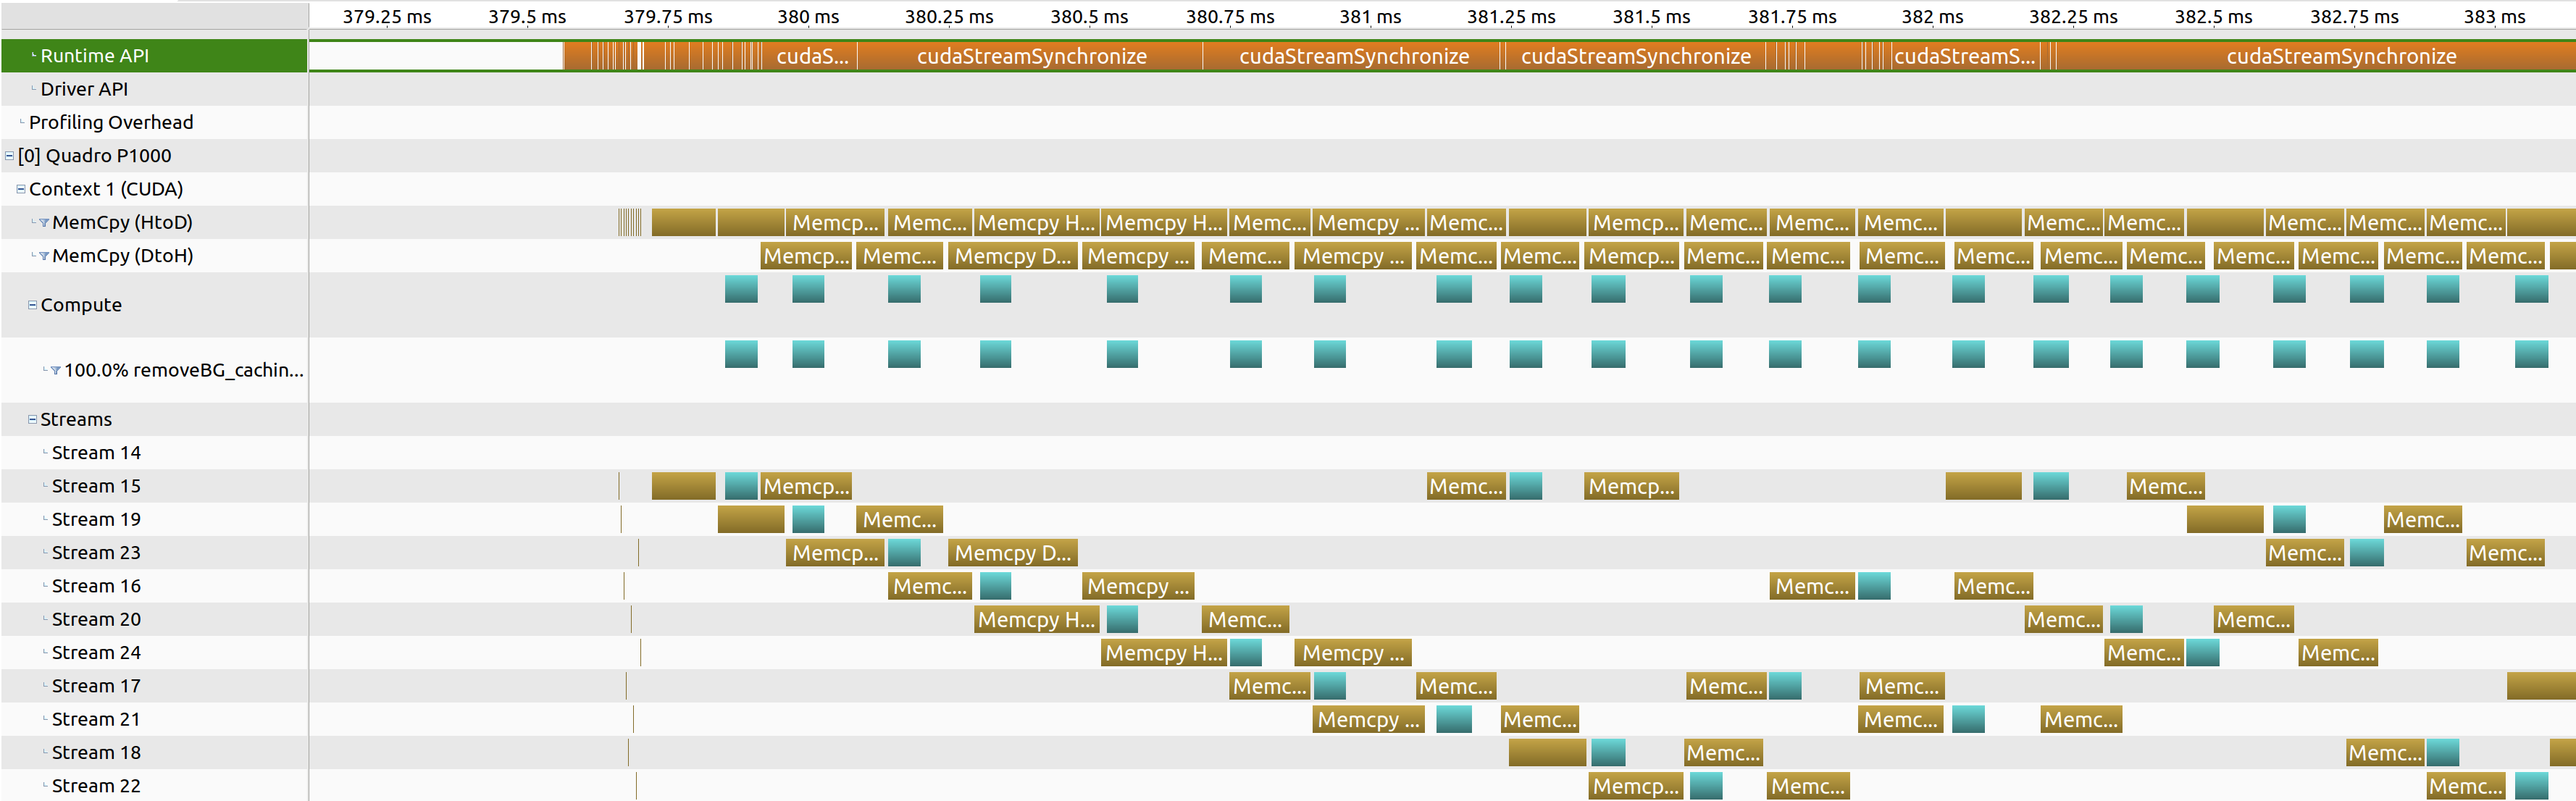
\includegraphics[width=\textwidth]{imgs/CudaStreamerFast.png}
\cite[CUDA Programming Guide, chapter 3.2.5.5ff]{cudaGuide}
\pagebreak

\section{Comparing different matrix multiplication kernels}
This snippet compares the total execution time of different matrix multiplication kernels. It provides also a class for easy measuring times in CPP.\\

The output of this snippet executed on a HP ZBook Studio G5 with a mobile Nvidia P1000 GPU is as followed:

Kernel Description:\\
\begin{tabular}{ll}
	Kernel 05: & Global Memory access kernel.\\
	Kernel 06A: & Shared memory with bursts for both tiles.\\
	Kernel 06B: & Shared memory with bursts for one tile.\\
	Kernel 06C & Shared memory with no bursts.\\
\end{tabular}


\texttt{Traditional Way: 1021.78ms. Value: 12812\\
	Kernel 05: 3.53315ms. Value: 12812\\
	Kernel 06A: 2.04691ms. Value: 12812\\
	Kernel 06B: 2.72592ms. Value: 12812\\
	Kernel 06C: 3.58989ms. Value: 12812 Slower because no burst transfers!"\\
}

But be aware compared to the nvidia-profiler output we see that this method is not very accurate for small kernels.

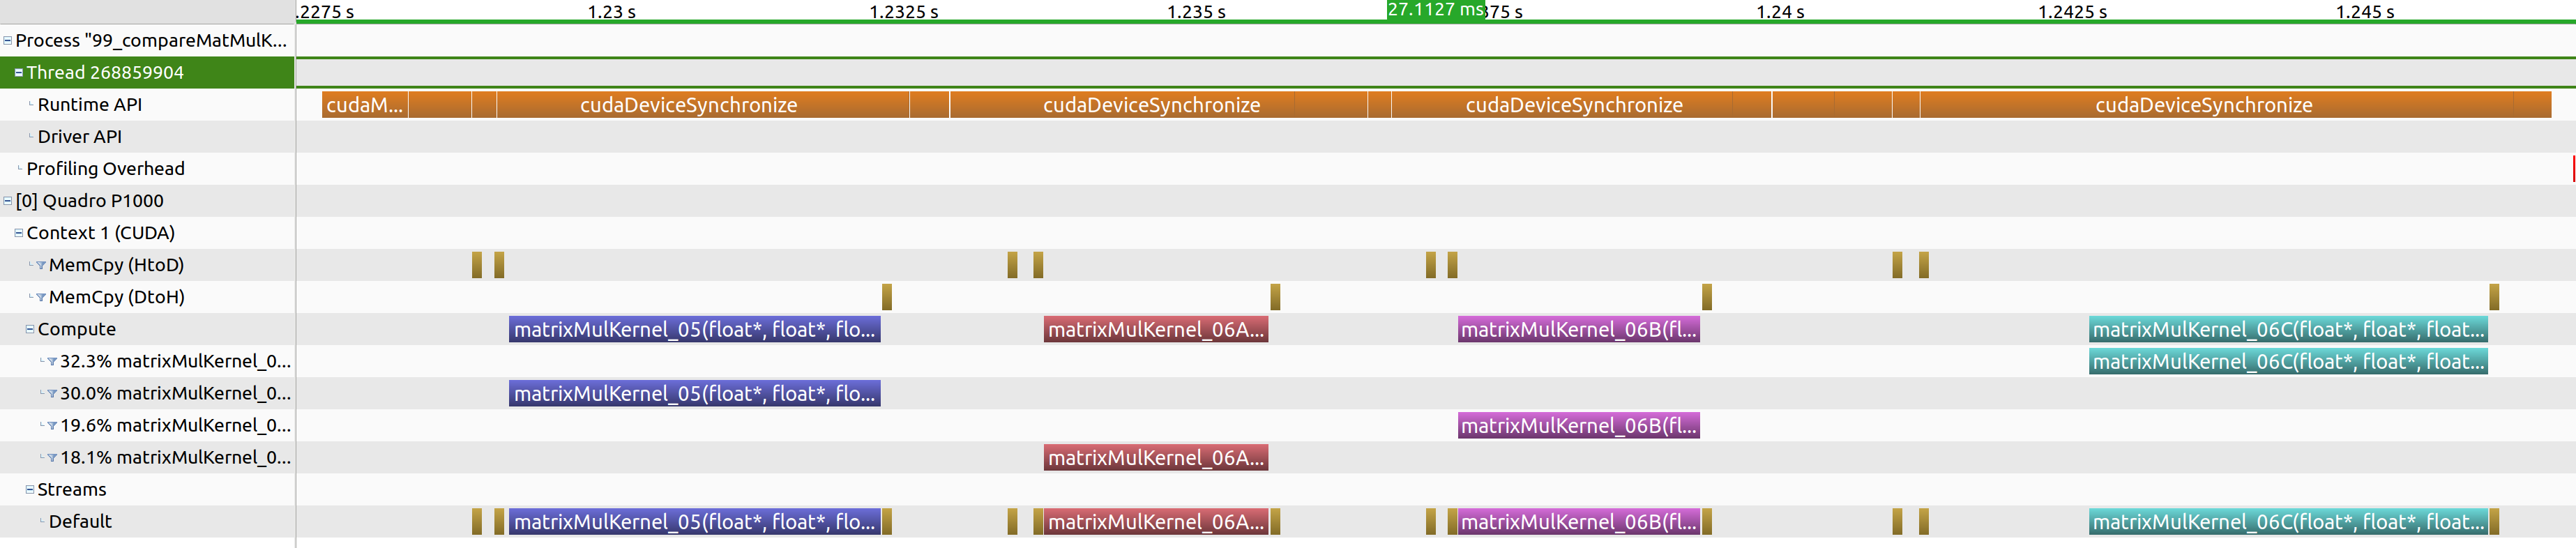
\includegraphics[width=\textwidth]{imgs/99_MatMulKernelComparison.png}

The readouts results from the tool are as followed:\\
\begin{tabular}{ll}
	Kernel 05: & 3.178ms\\
	Kernel 06A: & 1.92ms\\
	Kernel 06B: & 2.073ms\\
	Kernel 06C & 3.415ms\\
\end{tabular}

Here we can definitely see that the using of shared memory in combination with burst transfers for global memory access is important to speed up GPU processing! 
